\chapter{Antecedentes}
\label{cap:Antecedentes}
En este capítulo se exponen los conceptos de ciencias de la computación más importantes relacionados con este trabajo y una breve revisión de trabajos similares.\\

\section{Sistema Inteligente}
Un agente inteligente es aquel que emprende la mejor acción posible ante una situación dada. El campo de la inteligencia artificial~\cite{Russ06} se centra en construir sistemas inteligentes que piensan como humanos, actúan como humanos, piensan racionalmente y actúan racionalmente. Como se puede observar, los cuatro enfoques están divididos en dos grupos: el primero se centra en los humanos y el segundo en la racionalidad. Un agente es racional si hace lo correcto en base a su conocimiento. El enfoque humano debe ser una ciencia empírica mientras que el enfoque racional se basa en una combinación de matemáticas e ingeniería. Estos cuatro enfoques de la inteligencia artificial han coexistido a lo largo de la historia.\\
\begin{itemize}
\item{El enfoque de la prueba de Turing (Actuar como humanos).}\\

  La prueba de Turing tenía como objetivo proporcionar una definición operacional y satisfactoria de inteligencia. Una máquina superaría la prueba si el examinador no fuese capaz de distinguir si el evaluado es una persona o un computador mediante una secuencia de preguntas. Para superarla un computador debe ser capaz de procesar el lenguaje natural, representar el conocimiento, contar con razonamiento automático y aprendizaje automático.
\item{El enfoque del modelo cognitivo (Pensar como humanos).}\\

Para determinar si una máquina es capaz de pensar de forma similar a un humano primero debe conocerse un mecanismo para ver como piensan los humanos: la ciencia cognitiva, en cuyo campo interdisciplinar convergen modelos computacionales de inteligencia artificial y técnicas de psicología intentando comprender el funcionamiento de la mente humana.
\item{El enfoque de las \textit{leyes del pensamiento} (Pensar racionalmente).}\\

  El \textit{modus operandi} de la mente humana se rige por silogismos, que son esquemas de estructuras de argumentación mediante los que se llega a conclusiones correctas si se parte de premisas correctas.
\item{El enfoque del agente racional (Actuar racionalmente).}\\

  Un agente racional actúa intentando alcanzar el mejor resultado y, en caso de haber incertidumbre, el mejor resultado esperado.
\end{itemize}
La inteligencia artificial y por ende los sistemas inteligentes tienen aplicación en numerosos ámbitos como:
\begin{itemize}
\item{Resolución de problemas.}
\item{Teoría de juegos.}
\item{Robótica y automatización.}
\item{Procesamiento del lenguaje natural.}
\end{itemize}

\section{Problema de Satisfacción de Restricciones}
La programación por restricciones es una metodología software que permite resolver problemas de gran complejidad, típicamente NP. Esta metodología ha generado mucha expectación en el área de la inteligencia artificial desde la década de los 60, ya que tiene un gran potencial para la resolución de problemas reales. La idea básica de este tipo de programación permite declarar una serie de restricciones sobre el dominio del problema, para después dar con soluciones que satisfacen las anteriores restricciones de la forma más optima posible. Así, un problema de satisfacción de restricciones~\cite{Russ06} está caracterizado por:
\begin{itemize}
	\item Un conjunto de variables, donde cada variable toma variables en un dominio.
	\item Un conjunto de restricciones, que permite representar las posibles combinaciones de valores válidos de las variables.
	\item La solución al \gls{PSR} será la asignación de valores a las variables de forma que se satisfacen las restricciones y se alcanza el objetivo, representado típicamente como una función a optimizar.
\end{itemize}
Las restricciones se caracterizan por su \textbf{aridad}, que viene a ser el número de variables que involucra. Pudiendo ser unarias, si solo involucran una variable; binarias, si involucran dos variables; y n-arias, si involucran más de dos variables.\\
\section{Programación Lineal}
La programación lineal~\cite{Loom64} tiene como objetivo optimizaAdiooor una función lineal cuyas variables están sujetas a un conjunto de restricciones.
Se trata de un campo de la matemática muy efectivo para la resolución de este tipo de problemas. Históricamente, el concepto de programación lineal debe su nombre a John Von Neumann (1947), uno de los matemáticos más importantes del siglo XX gracias a sus contribuciones en las ciencias de la computación; y a George Dantzig (1947), cuyo trabajo intentaba asignar 70 puestos de trabajo a 70 personas mediante programación lineal. Las permutaciones necesarias para la asignación óptima de dichos puestos era igual al factorial de 70 (70!). Curiosamente, mediante programación lineal el problema se resuelve de manera eficiente pues el número de combinaciones se reduce en su mayor parte. La programación lineal puede ser aplicable a numerosos problemas comunes tales como:
\begin{itemize}
\item Asignación de horarios a profesores en un centro educativo para obtener la mayor productividad a la par que comodidad para profesor y alumno.
\item Distribución de elementos en almacenes de tal modo que se reduzca el costo de almacenamiento teniendo en cuenta la capacidad limitada.
\item Distribución de bienes entre compradores y consumidores de tal modo que las ganancias del intermediario sean máximas.
\end{itemize}
Como se puede observar, el problema de este \gls{TFG} está muy relacionado con el último ejemplo, pues se distribuye cantidad de energía entre fuentes de entrada y fuentes de salida de manera óptima para garantizar un gasto mínimo de consumo energético.\\

En un problema de programación lineal puede ocurrir que:
\begin{itemize}
\item Exista una solución óptima.
\item Existan varias soluciones óptimas.
\item No exista solución.
\item Existan infinitas soluciones.
\end{itemize}
La situación deseada es la primera, pero puede ocurrir alguno de los otro casos. Estas situaciones pueden resolverse convirtiendo las restricciones que son inecuaciones (desigualdades) en igualdades.\\

Existen varios métodos de programación lineal. El más utilizado es el conocido como el \textbf{método Simplex}, que se basa en evaluar solo algunos puntos extremos mediante dos condiciones:
\begin{itemize}
\item \textbf{Optimalidad}. La solución inferior relativa al punto de solución actual no se tiene en cuenta.
  \item \textbf{Factibilidad}. Una vez se encuentra una solución básica factible, sólo apareceran soluciones factibles.
\end{itemize}
Otro método de programación lineal es el método de ramificación y acotamiento \textit{branch and bound}, el cuál divide el problema en varios subproblemas de programación lineal, acotamiento que permite obtener soluciones óptimas que se mejoran por cada subproblema.\\

\section{Trabajos relacionados}
Tal y como se ha comentado en el Capítulo~\ref{cap:Introduccion}, existe una gran demanda energética que desemboca en un encarecimiento de la energía eléctrica. Esto hace que sea una problemática en la que se ha trabajado tanto en el ámbito comercial como en la investigación.\\

En el ámbito de la investigación se han encontrado varios estudios relacionados. Uno de ellos es una tesis doctoral perteneciente a la Universidad de Alicante: ``Modelado y simulación de la distribución de energía eléctrica en sistemas genéricos consistentes en diversas fuentes y múltiples modos de transmisión''~\cite{Valdi13}. El trabajo de investigación de esta tesis doctoral aborda el problema de la distribución eléctrica en sistemas genéricos con varias fuentes de energía (eólica, hidroeléctrica, solar, etc). En este caso el sistema se implementa como un sistema multiagente en el que existen, cooperan y se comunican agentes que representan las fuentes energéticas, los consumos y los servicios. En la Figura~\ref{fig:tesis} se muestra la interfaz de usuario de este sistema, donde mediante unos parámetros de configuración se realiza la distribución de energía entre cada uno de los agentes involucrados.\\
\begin{figure}[H]
	\centering
	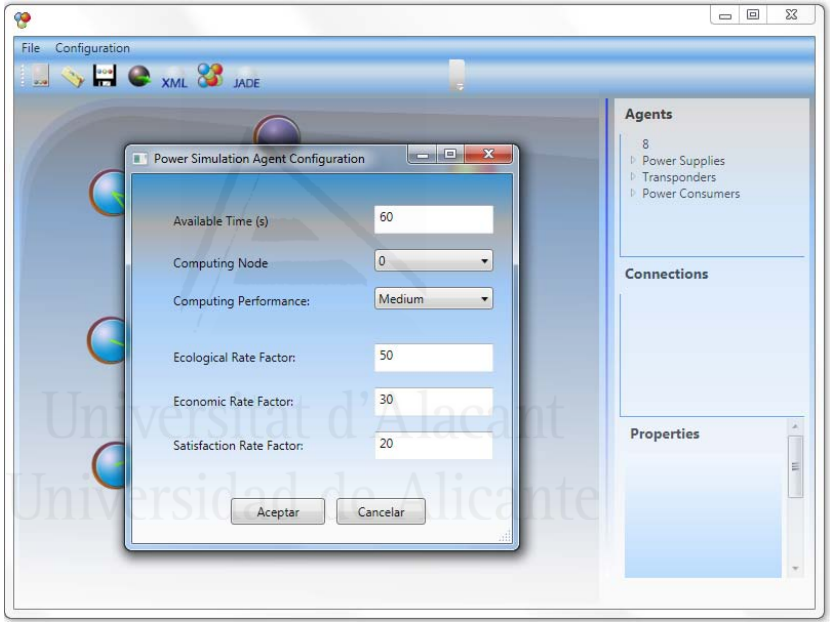
\includegraphics[width=10cm]{figs/tesis.png}
	\caption{Formulario de optimización de la aplicación perteneciente a~\cite{Valdi13}}
        \label{fig:tesis}
\end{figure}

En el ámbito comercial, existen varias aplicaciones móviles y web relacionadas con esta temática. A continuación se exponen algunas de ellas:
\begin{itemize}
  \item \textbf{Mi.Luz}~\cite{MiLu}: Se trata de una aplicación móvil disponible para iOS y Android que permite conocer el precio del KWh en cada momento del día, para que así el usuario establezca el consumo eléctrico en su hogar.(Figura~\ref{fig:miluz}).
    \begin{figure}[!h]
	\centering
	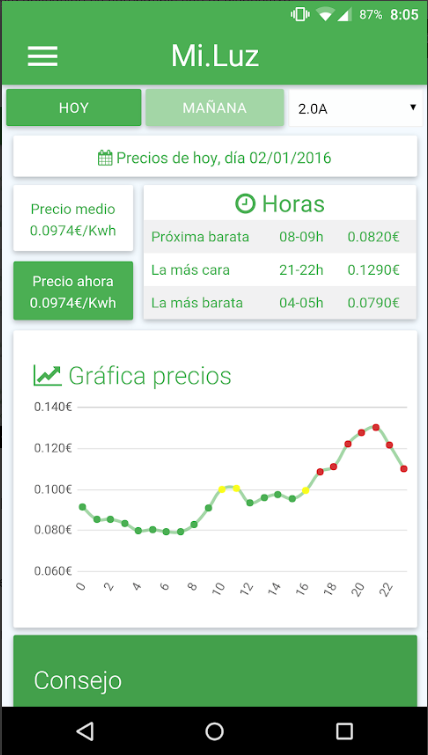
\includegraphics[width=4cm]{figs/miluz.png}
	\caption{Dashboard de la aplicación Mi.Luz}
        \label{fig:miluz}
\end{figure}
\item \textbf{Área Personal - Endesa}~\cite{End}: Endesa brinda a sus clientes un área personal donde permite consultar el consumo realizado en un día determinado en su hogar, desglosado en horas. Además permite la descarga de ficheros con el consumo del hogar. Esta funcionalidad será de utilidad en este \gls{TFG}.
\item \textbf{Virtual Energy Advisor}~\cite{Vea}: Aplicación ganadora del premio \textit{Barcelona Smart City App Hack}. Mediante la introducción de facturas del hogar y perfil, la aplicación ofrece información adaptada en tiempo real, previsiones de consumo y alertas en las horas de menor precio.
\item \textbf{Mirubee}~\cite{MiRu}: Es una aplicación móvil disponible para iOS y Android. Mediante la instalación de un medidor inteligente en el cuadro eléctrico del hogar, la aplicación analiza el patrón de consumo que se produce y a partir de ello proporciona indicaciones personalizadas para ahorrar en la factura de la luz. Mirubee fue creado por una \textit{start-up} española en 2011 con el objetivo de facilitar la monitorización de energía en las casas mediante una plataforma de prestaciones profesionales (Figura~\ref{fig:mirubee}).
  \begin{figure}[!h]
	\centering
	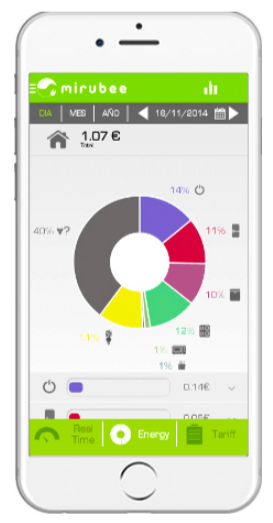
\includegraphics[width=4cm]{figs/mirubee.png}
	\caption{Informe de consumo del hogar en Mirubee}
        \label{fig:mirubee}
\end{figure}
\end{itemize}
